% Pro kompilaci po částech (viz projekt.tex), nutno odkomentovat a upravit
%\documentclass[../projekt.tex]{subfiles}
%\begin{document}

\chapter{Úvod}

\chapter{Vizualizácia dát z~mobilných mapovacích systémov}

Výstupom mobilného mapovacieho systému je množstvo dát z rôznych senzorov. Dáta, ktoré boli poskytnuté k tvorbe tejto práce, obsahovali v prvom rade mračná bodov získané z lidaru. Aby bolo možné s týmito mračnami bodov pracovať a vhodne ich zobrazovať, je potrebné, aby mobilný mapovací systém zaznamenával údaje o svojej polohe. V tomto prípade boli k dispozícii údaje o transláciách a rotáciách kamery s časovými razítkami. Ďalej býva súčasťou mobilného mapovacieho systému klasická kamera. Pre zobrazenie mračna bodov takým spôsobom, aby sa zobrazenie čo najviac zhodovalo s kamerovým záznamom, je nutné poznať parametre kamery -- kalibračnú maticu a prípadne aj parametre skreslenia.

Pri vývoji aplikácie, ktorá má umožniť vizualizáciu týchto dát a navyše aj ďalších vektorových dát, je nutné poznať základné princípy zobrazovania 3D dát v počítačovej grafike. Ďalej je potrebné vybrať si a naštudovať technológie, pomocou ktorých bude aplikácia vytvorená, a to konkrétne niektorý z frameworkov pre tvorbu aplikácií v jazyku Python a vhodný framework pre zobrazenie grafických dát. Práve to je predmetom tejto kapitoly.

\section{Dierkový model kamery -- teoretický základ perspektívneho zobrazenia}

Kamera je v~počítačovej grafike pojem, ktorý označuje projekciu bodov z~trojrozmerného priestoru do roviny. Túto projekciu je možné vyjadriť pomocou matíc a je väčšinou bodová (\emph{central projection}).

Existuje niekoľko rôznych modelov kamery, z~ktorých najjednoduchší je dierkový model kamery (\emph{pinhole camera model}). U~tohto modelu je stred projekcie $\mathbf{C}$  (\emph{camera centre}) v~počiatku Euklidovského súradnicového systému a body sa premietajú do roviny $z = f$, ktorá sa označuje ako obrazová rovina (\emph{image plane}).

Princíp zobrazenia je nasledovný: obrazom bodu $\mathbf{X} = (X, Y, Z)^T$ je bod $\mathbf{x}$, kde priamka vedúca bodom $\mathbf{X}$ a stredom projekcie $\mathbf{C}$ pretína obrazovú rovinu (obrázok \ref{fig:model_kamery1}). Z~podobnosti trojuholníkov je možné odvodiť, že bod $\mathbf{x}$ má súradnice $(fX/Z, fY/Z, f)^T$, postup je naznačený na obrázku \ref{fig:model_kamery2}.

\begin{figure}[h!]
    \centering
    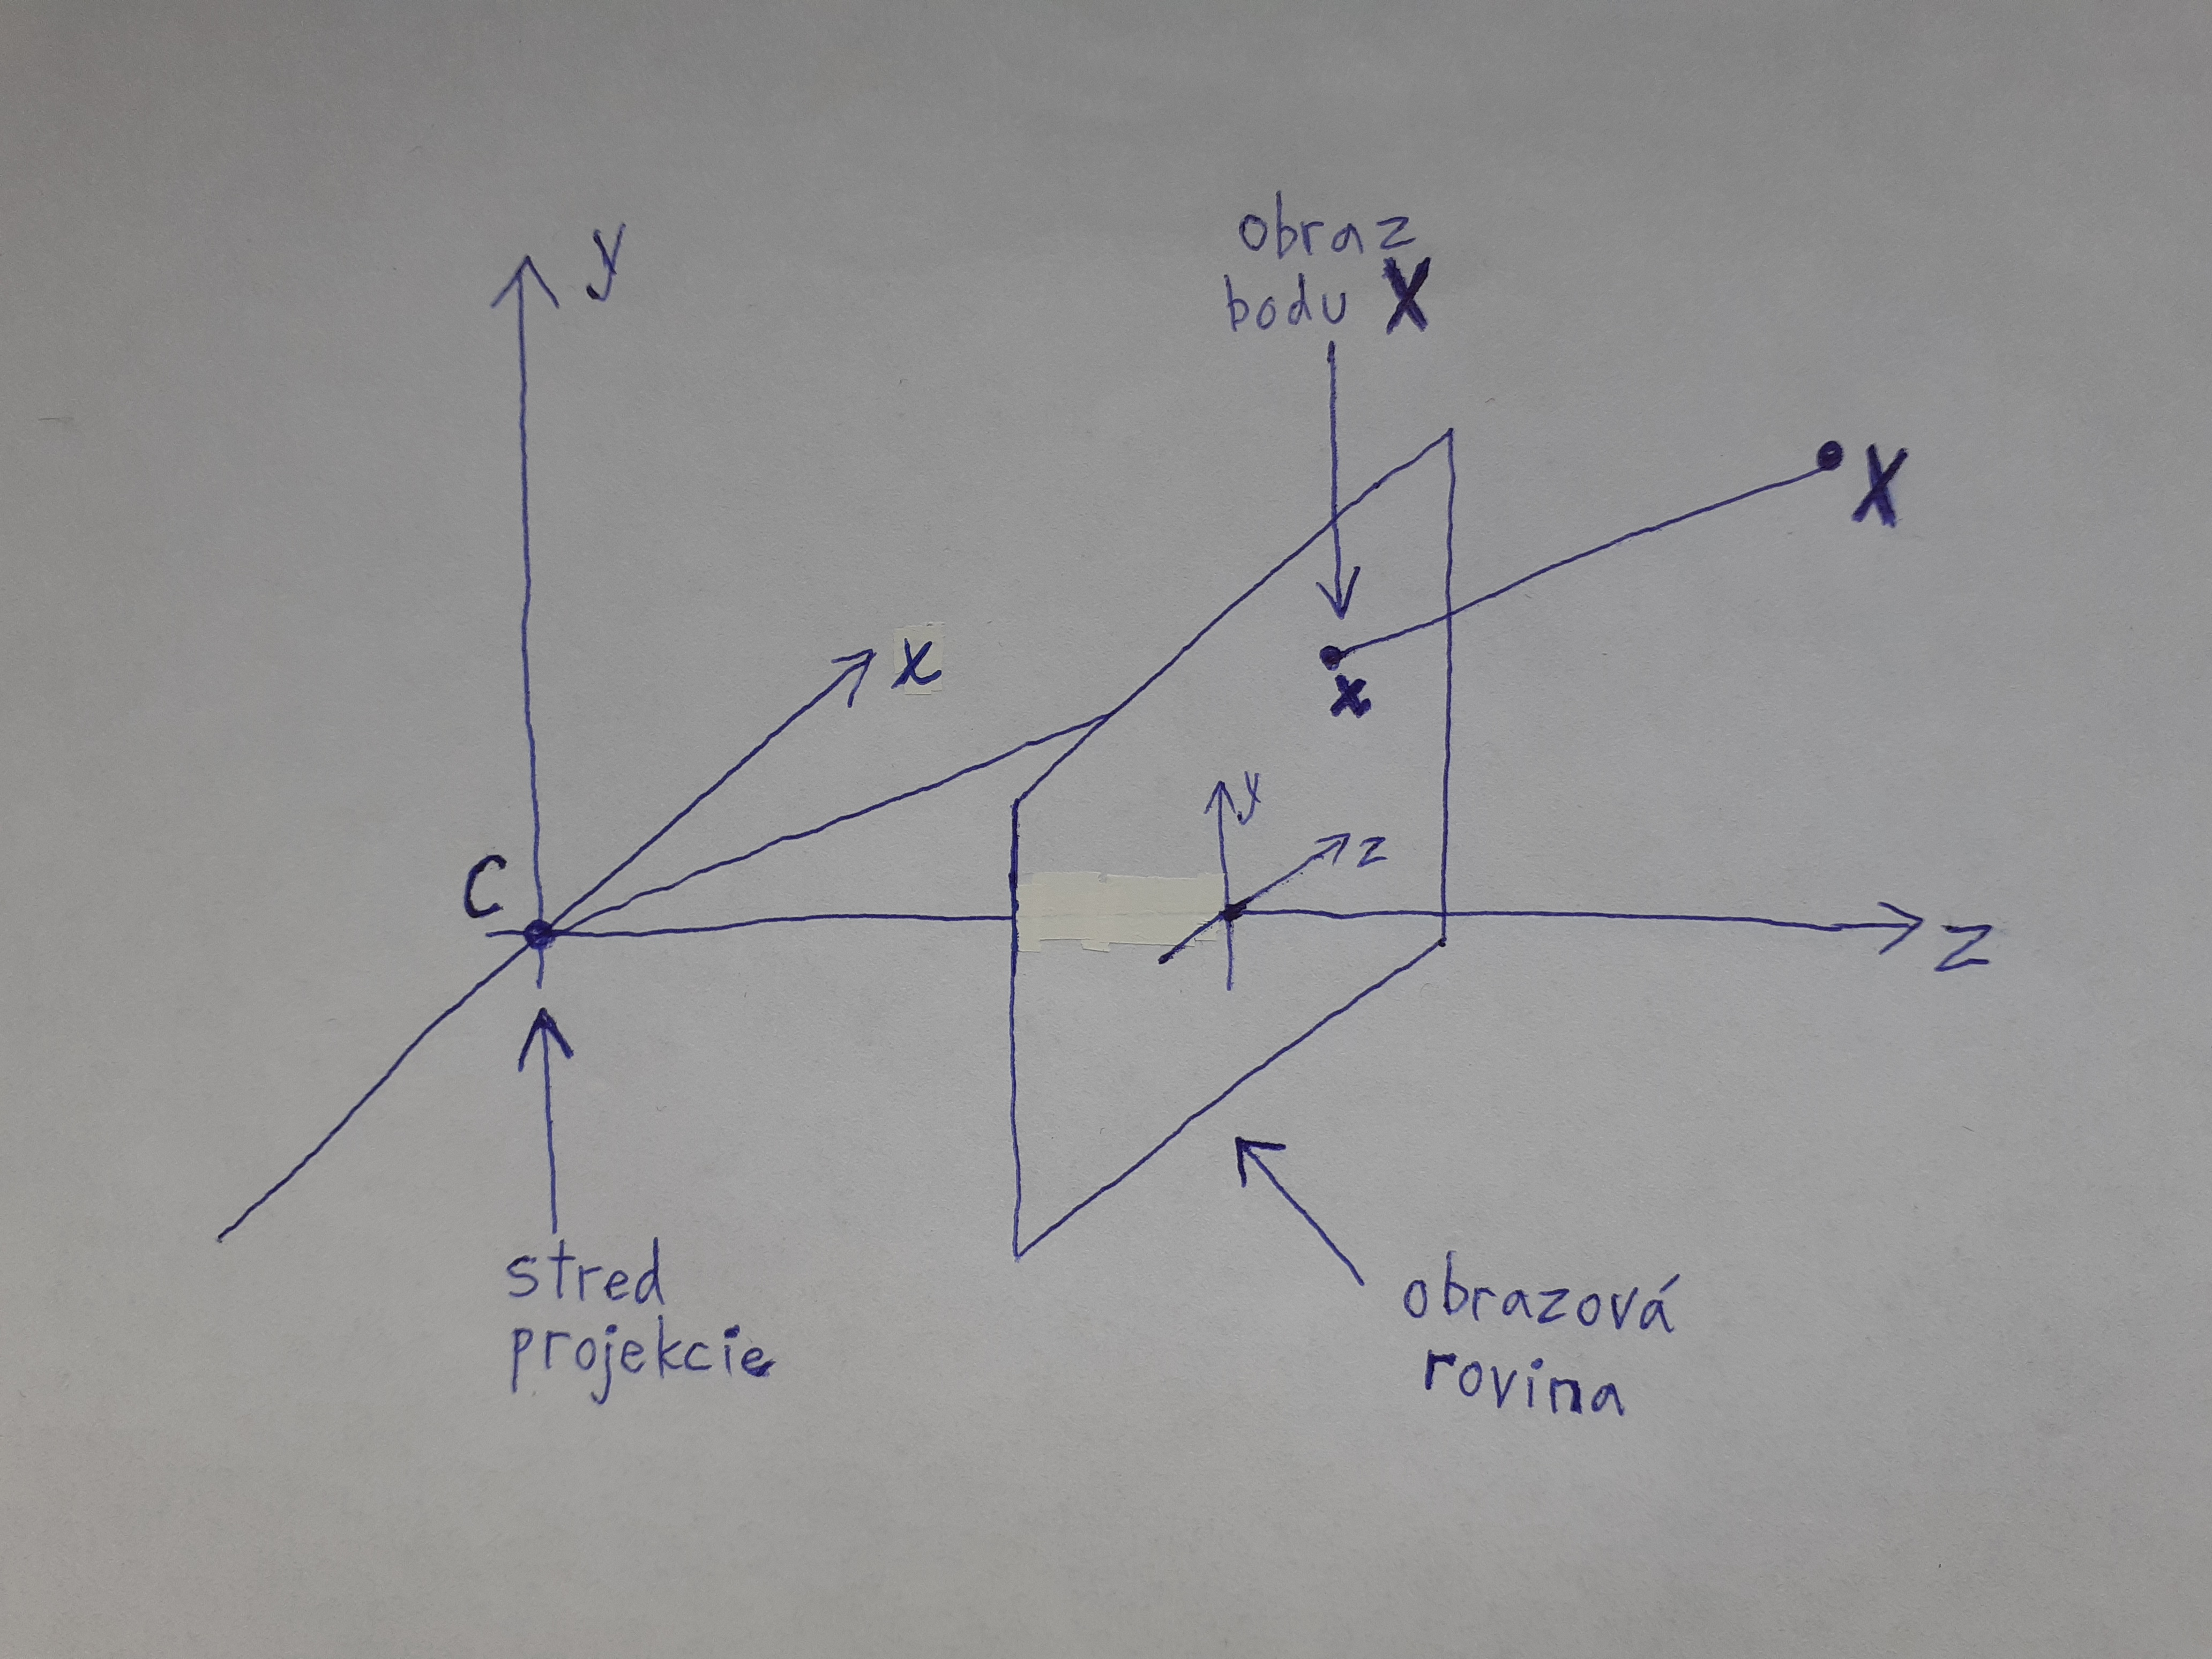
\includegraphics[width=0.7\linewidth]{text_prace/obrazky-figures/model_kamery1.jpg}
    \caption{[TODO: prekresliť] Zakladný princíp dierkového modelu kamery.}
    \label{fig:model_kamery1}
\end{figure}

\begin{figure}[h!]
    \centering
    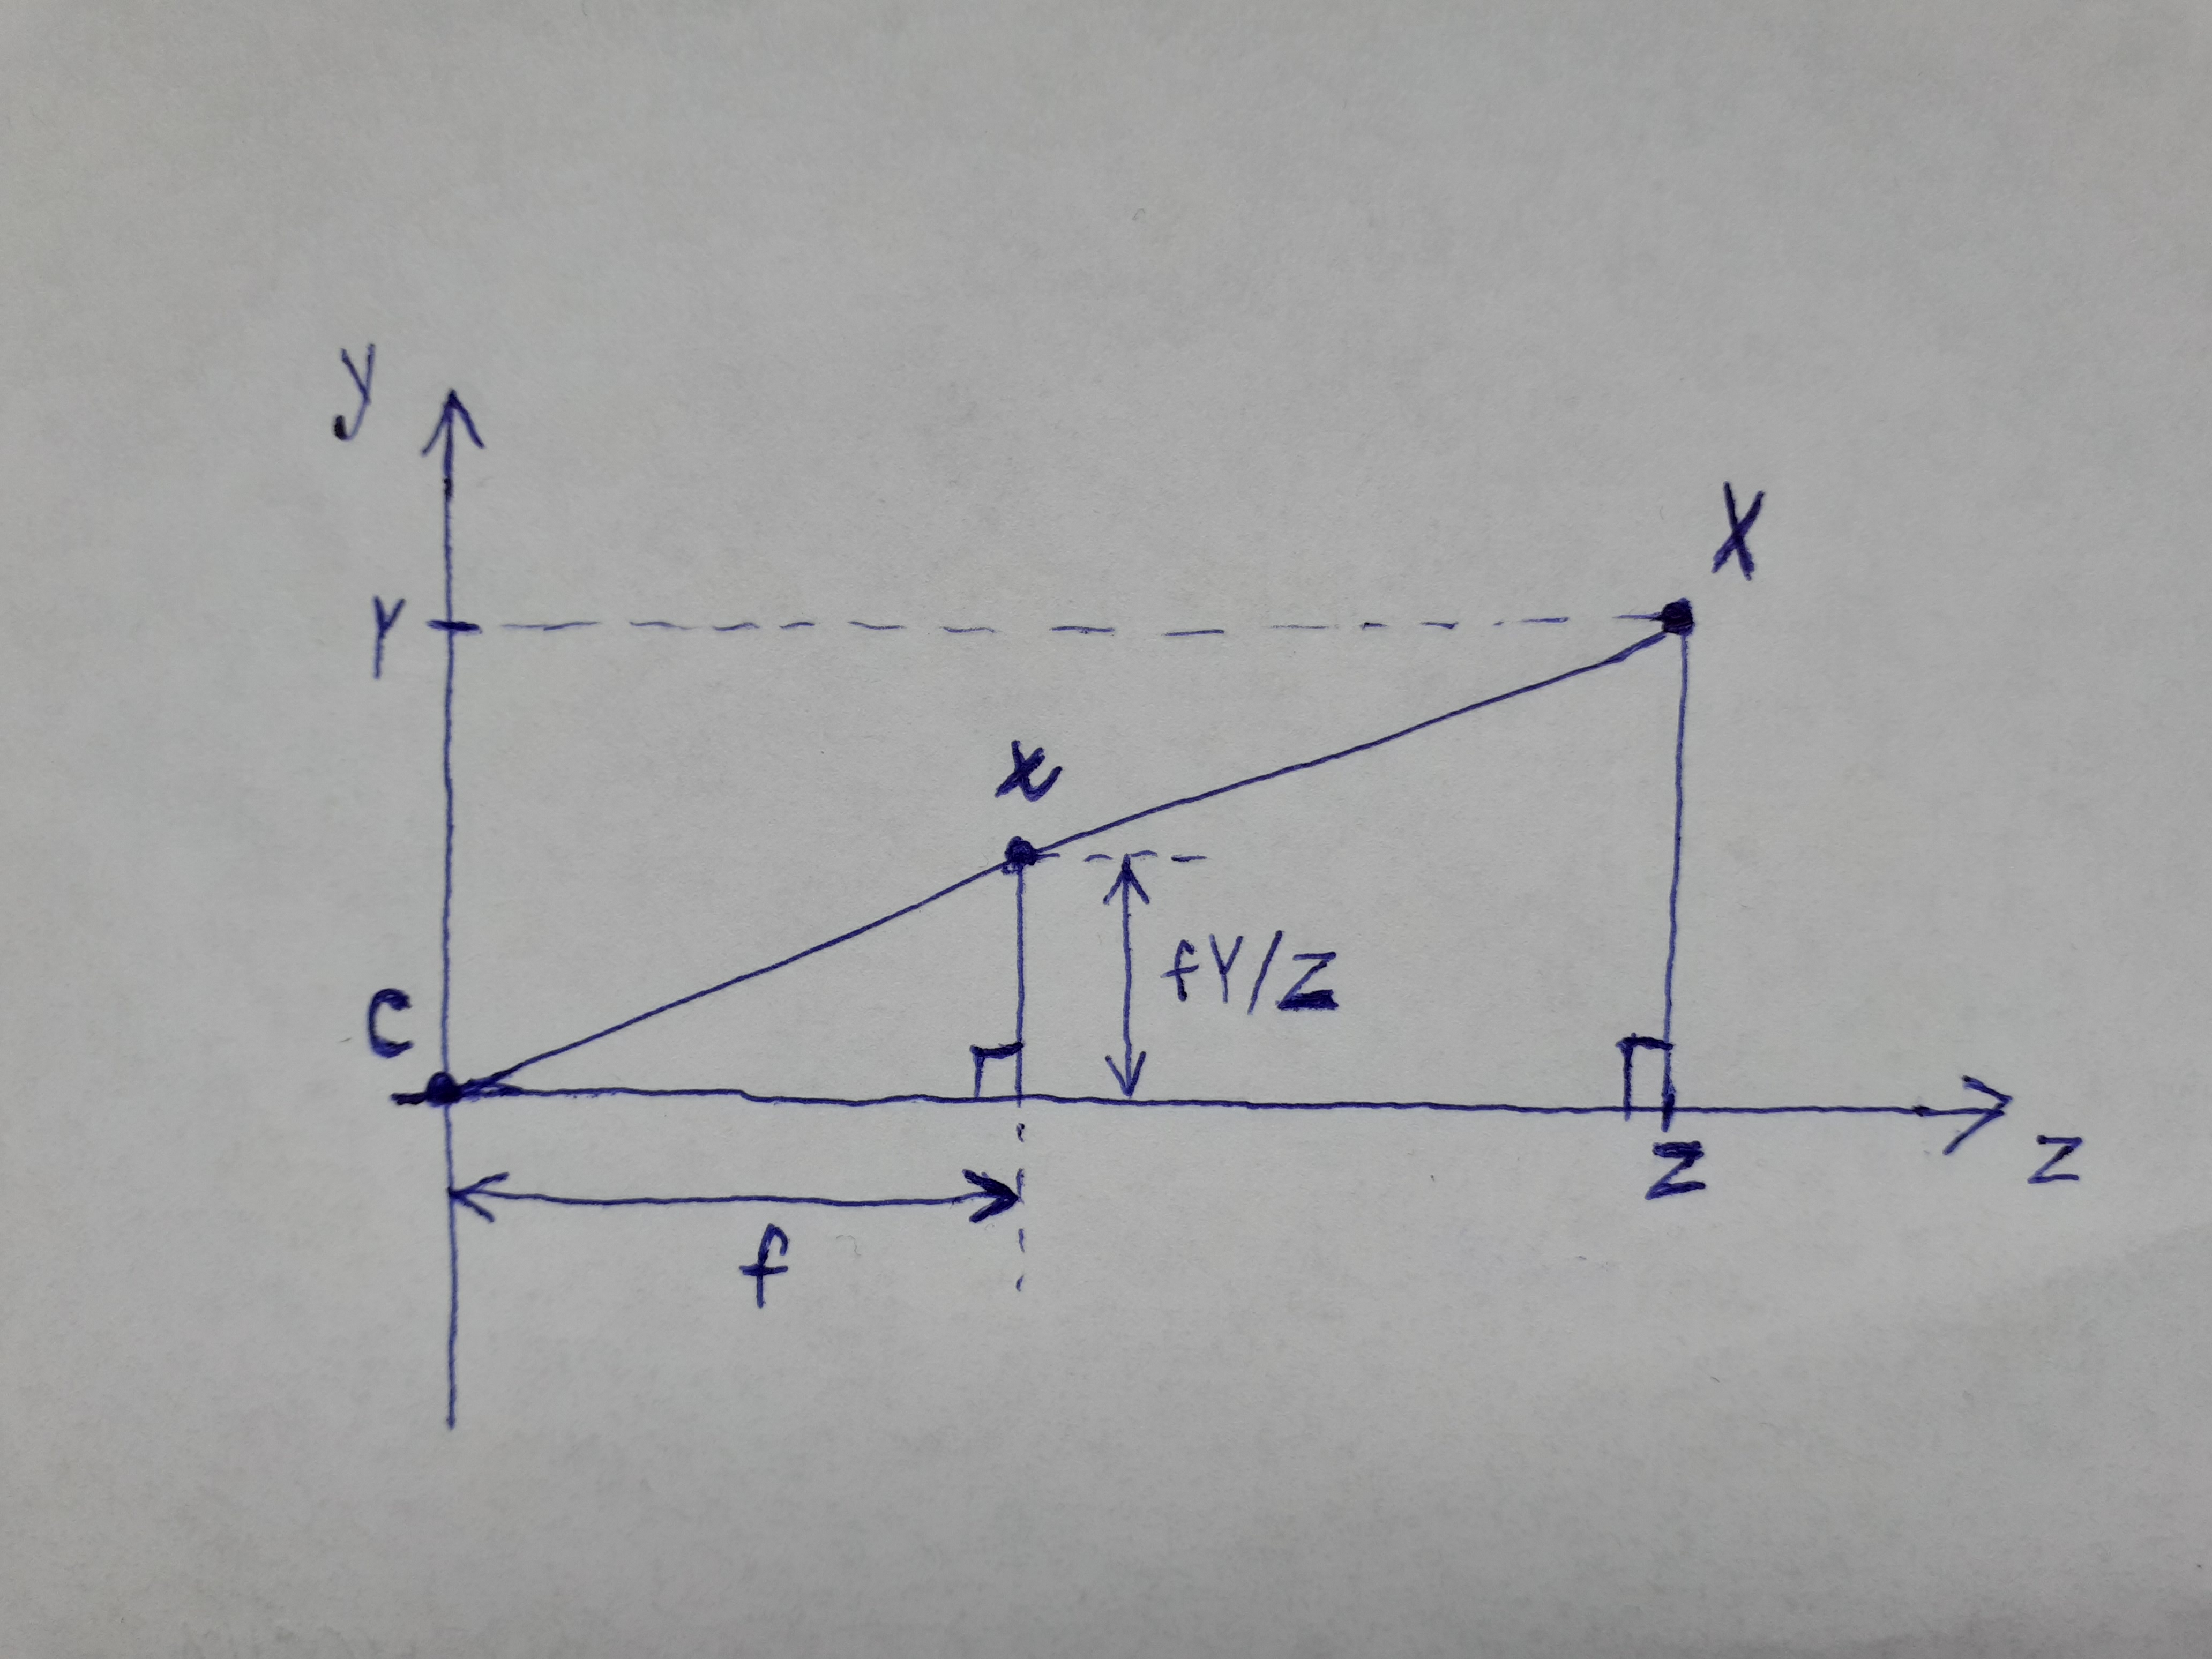
\includegraphics[width=0.7\linewidth]{text_prace/obrazky-figures/model_kamery2.jpg}
    \caption{[TODO: prekresliť] Náčrt odvodenia súradníc bodu $\mathbf{x}$.}
    \label{fig:model_kamery2}
\end{figure}

Keďže všetky obrazy bodov ležia v~obrazovej rovine $z = f$, je možné poslednú súradnicu zanedbať a zapisovať súradnice bodu $\mathbf{x}$ v~súradnicovom systéme obrazovej roviny ako $(fX/Z, fY/Z)^T$.

Túto projekciu môžeme v~homogénnych súradniciach zapísať pomocou násobenia matíc nasledovným spôsobom:

$$ \mathbf{x} 
=
\begin{pmatrix}
fX \\
fY \\
Z
\end{pmatrix}
=
\begin{bmatrix}
f &   &   & 0 \\
  & f &   & 0 \\
  &   & 1 & 0
\end{bmatrix}
\begin{pmatrix}
X \\
Y \\
Z \\
1
\end{pmatrix}
=
\begin{bmatrix}
f &   &   & 0 \\
  & f &   & 0 \\
  &   & 1 & 0
\end{bmatrix}
\mathbf{X}
=
\mathrm{P} \mathbf{X}
$$

Maticu $\mathrm{P}$ nazývame projekčnou maticou kamery (\emph{camera projection matrix}).

\subsubsection{Rozšírenia základného dierkového modelu kamery}

V~praxi väčšinou chceme vyjadriť body na obrazovej rovine v~súradnicovom systéme, ktorý nemá stred v~bode $(0, 0, f)^T$, ale v~ľubovoľnom bode $(-p_x, -p_y, f)^T$ (obrázok \ref{fig:model_kamery3}). Obrazom bodu $\mathbf{X} = (X, Y, Z)^T$ (v~súradnicovom systéme kamery) potom bude bod $\mathbf{x} = (fX/Z + p_x, fY/Z + p_y, f)^T$ (v~súradnicovom systéme obrazovej roviny). To je možné zahrnúť do projekčnej matice nasledovným spôsobom:

$$ \mathrm{P} =
\begin{bmatrix}
f &   & p_x & 0 \\
  & f & p_y & 0 \\
  &   &  1  & 0
\end{bmatrix}
$$

$$ \mathbf{x} 
=
\begin{pmatrix}
fX/Z + p_x \\
fY/Z + p_y \\
1
\end{pmatrix}
=
\begin{pmatrix}
fX + Z p_x \\
fY + Z p_y \\
Z
\end{pmatrix}
=
\begin{bmatrix}
f &   &  p_x & 0 \\
  & f &  p_y & 0 \\
  &   &   1  & 0
\end{bmatrix}
\begin{pmatrix}
X \\
Y \\
Z \\
1
\end{pmatrix}
$$

Maticu

$$ \mathrm{K} 
=
\begin{bmatrix}
f &   &  p_x \\
  & f &  p_y \\
  &   &   1  
\end{bmatrix}
$$

nazývame kalibračnou maticou kamery (\emph{camera calibration matrix}) a medzi ňou a projekčnou maticou platí vzťah
$\mathrm{P} = \begin{bmatrix} \mathrm{K} | 0 \end{bmatrix}$, kde $0$ predstavuje nulový stĺpcový vektor.

\begin{figure}[h!]
    \centering
    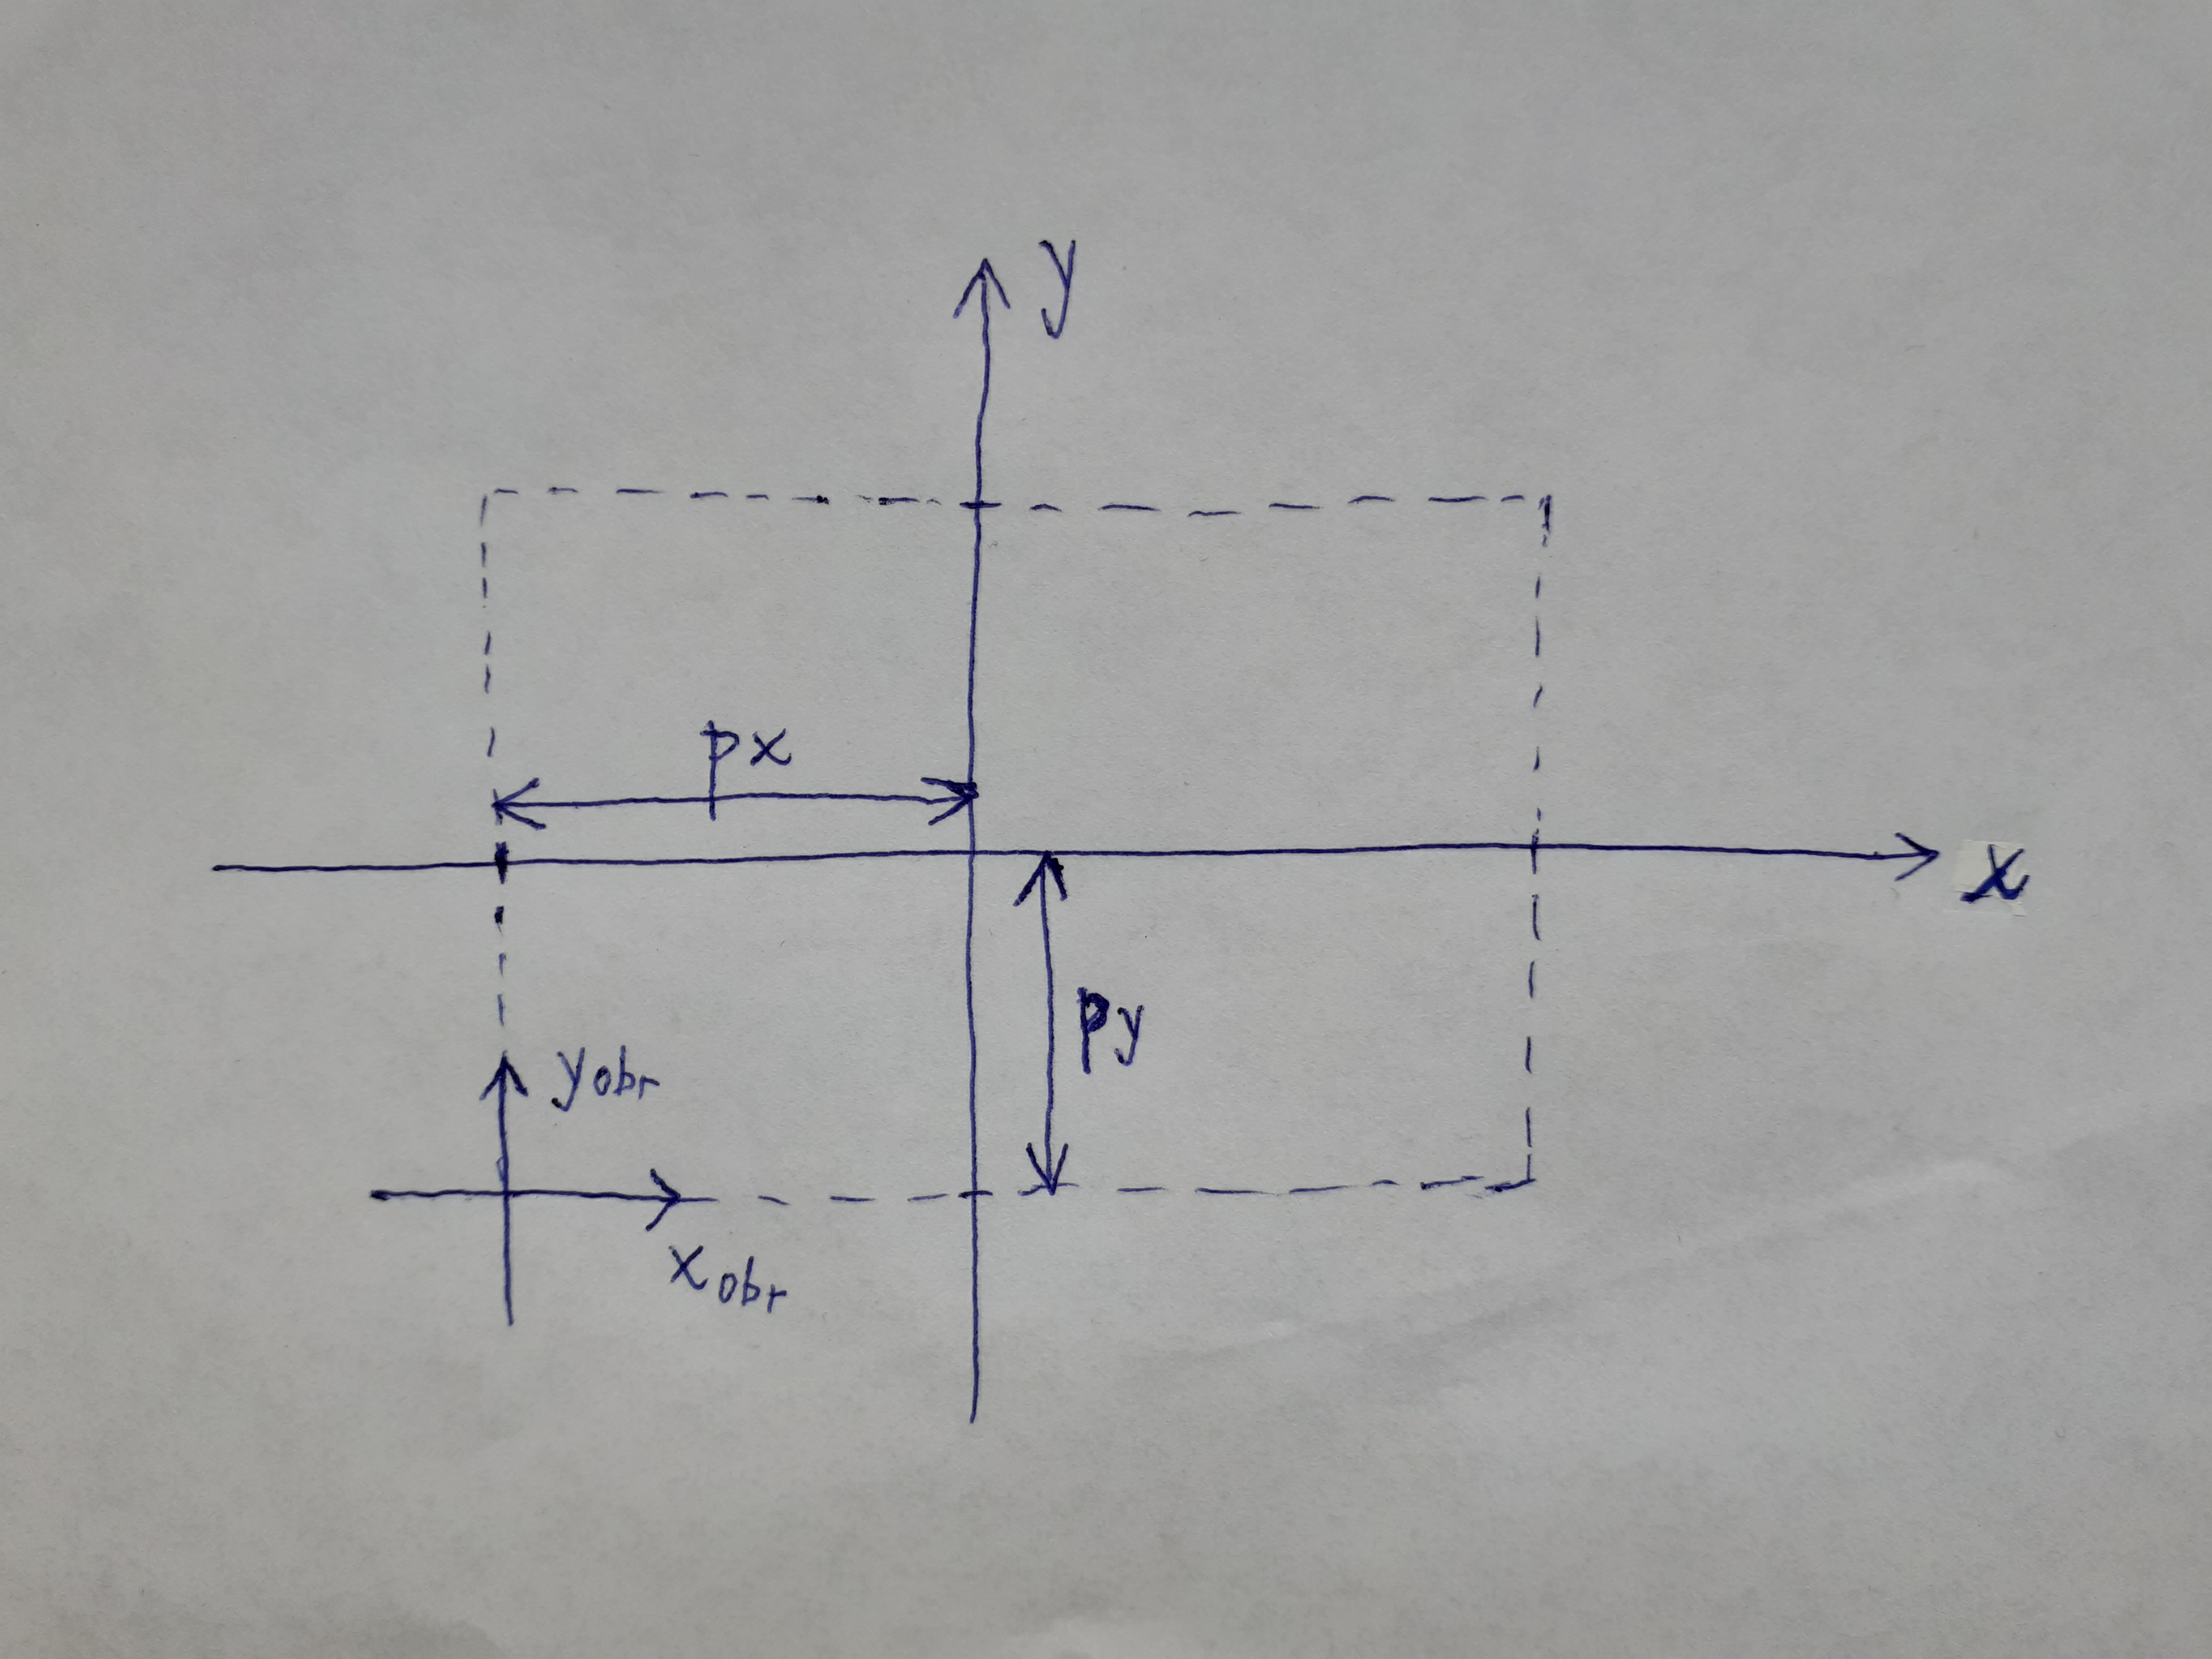
\includegraphics[width=0.7\linewidth]{text_prace/obrazky-figures/model_kamery3.jpg}
    \caption{[TODO: prekresliť] Súradnicový systém so stredom v~bode $(-p_x, -p_y, f)^T$ obrazovej roviny.}
    \label{fig:model_kamery3}
\end{figure}


Parametre $f$, $p_x$ a $p_y$ označujeme ako \textbf{vnútorné parametre kamery}.

Až doteraz sme predpokladali, že kamera má stred v~počiatku súradnicovej sústavy a je \uv{otočená} v~smere osi $z$, t. j. že obrazová rovina je rovnobežná s~rovinou $xy$. V~praxi to tak však nebýva a kamera má v~súradnicovom systéme, v~ktorom sú definované zobrazované body, istú rotáciu a transláciu. V~takom prípade rozlišujeme všeobecný súradnicový systém a súradnicový systém kamery (\emph{world coordinate frame} a \emph{camera coordinate frame}).

Ak $\widetilde{\mathbf{X}}$ je vektor súradníc bodu $\mathbf{X}$ vo všeobecnom súradnicovom systéme a vektor $\widetilde{\mathbf{X}}_{\mathrm{cam}}$ reprezentuje ten istý bod v~súradnicovom systéme kamery, tak platí vzťah 
$$\widetilde{\mathbf{X}}_{\mathrm{cam}} = \mathrm{R} (\widetilde{\mathbf{X}} - \widetilde{\mathbf{C}}),$$ 
kde $\widetilde{\mathbf{C}}$ sú súradnice stredu kamery vo všeobecnom súradnicovom systéme a $\mathrm{R}$ je rotačná matica $3 \times 3$ reprezentujúca orientáciu súradnicového systému kamery. To vedie k~novému vyjadreniu projekčnej matice ako $\mathrm{P} = \mathrm{K} \mathrm{R} \bigl[ \mathrm{I} | - \widetilde{\mathbf{C}} \bigr]$, kde $\mathrm{I}$ je jednotková matica $3 \times 3$.

Parametre $\mathrm{R}$ a $\widetilde{\mathbf{C}}$ označujeme ako \textbf{vonkajšie parametre kamery}.

Zdrojom všetkých informácií, ktoré boli uvedené v~tejto sekcii, je kniha \emph{Multiple View Geometry in Computer Vision} od autorov R. Hartley a A. Zisserman \cite{multiple_view_geometry}.

\section{Existujúce možnosti zobrazenia dát z~mobilných mapovacích systémov v~jazyku Python}

\subsubsection{Framework deck.gl a jeho nadstavba Pydeck}
\label{sec:deck_gl}

Javascriptový framework deck.gl je určený na zobrazovanie dát najmä na mapových podkladoch. Vyznačuje sa vysokou presnosťou a výkonnosťou. Pre akceleráciu využíva rozhrania WebGPU a WebGL2 \cite{deck.gl_documentation}.

Vizualizácia dát v~deck.gl sa skladá z~dvoch základných častí:
\begin{itemize}
    \item Vrstvy (\texttt{Layers}). Do vrstiev sa ukladajú zobrazované dáta. Framework deck.gl ponúka vyše 30 preddefinovaných typov vrstiev. Pre túto prácu je významná najmä vrstva \texttt{PointCloudLayer}, ktorá je určená na zobrazenie mračna bodov, a vrstva \texttt{LineLayer}, ktorá je určená na zobrazenie čiar.
    \item Pohľad (\texttt{View}). Definuje vlastnosti kamery, napríklad zorné pole a prednú a zadnú orezávaciu rovinu (\emph{near plane} a \emph{far plane}).
    Časť \texttt{ViewState} určuje polohu a orientáciu kamery. Typ pohľadu definuje spôsob interakcie vizualizácie s~používateľom, napríklad pre zobrazenie trate z~pohľadu strojvedúceho je ideálny typ \texttt{FirstPersonView}.
\end{itemize}

Hoci je framework deck.gl primárne určený pre použitie v~Javascripte, je možné ho použiť aj v~jazyku Python, a to pomocou knižnice \textbf{Pydeck}. Tá je pomerne jednoduchá a podstatou jej činnosti je, že prevedie kód napísaný v~jazyku Python do formátu JSON. Framework deck.gl má totiž modul @deck.gl/json, ktorý prijíma reprezentáciu vizualizácie vo formáte JSON a transformuje ju do javascriptového kódu (na definície funkcií a deck.gl objektov)\footnote{Ukážka rozhrania modulu @deck.gl/json je na \url{https://deck.gl/playground}.}.

Knižnica Pydeck je dobrým prostriedkom na vytvorenie jednoduchých vizualizácií, s~ktorými môže používateľ interagovať pohybmi myši. Jej možnosti sú však oproti pôvodnému frameworku deck.gl veľmi obmedzené. Nie je vhodná na vytváranie zložitejších animácií s~veľkým množstvom dát, pretože sa aj po tej najmenšej zmene musia dáta a definícia vizualizácie nanovo prevádzať do formátu JSON a následne na javascriptový kód (obrázok \ref{fig:pydeck_dashdeck_schema}), čo je veľmi časovo náročné.

\begin{figure}[h]
    \centering
    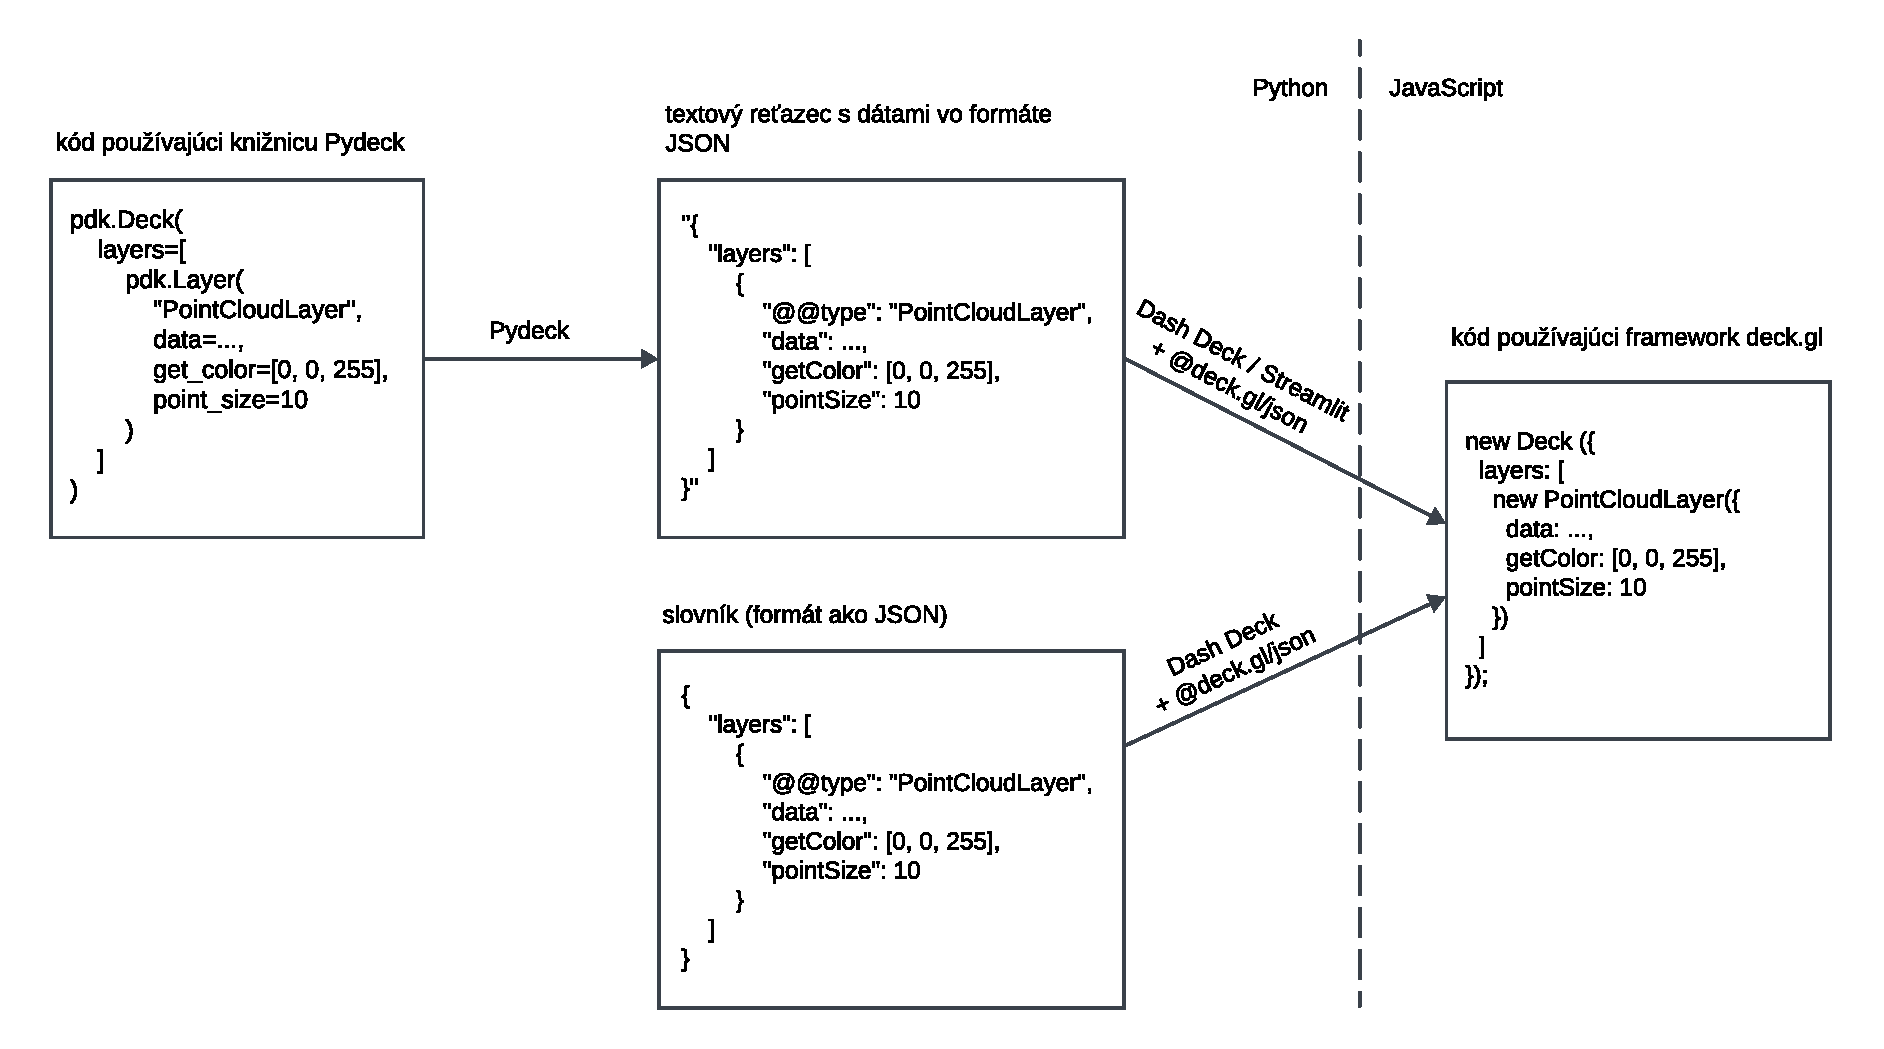
\includegraphics[width=1\linewidth]{text_prace/obrazky-figures/pydeck_dashdeck_transformacie.pdf}
    \caption{Schéma vzťahov medzi technológiami Pydeck, Dash Deck a deck.gl a transformácií, ktorými prechádza definícia zobrazenia.}
    \label{fig:pydeck_dashdeck_schema}
\end{figure}

\section{Frameworky pre tvorbu interaktívnej webovej aplikácie v~jazyku Python}

\subsubsection{Porovnanie frameworkov Streamlit a Dash}

Streamlit a Dash sú frameworky, ktoré majú rovnaké zameranie: oba slúžia na tvorbu webových aplikácií pre prácu s~dátami (\emph{data apps}) v~jazyku Python. Dash je oproti Streamlitu na nižšej úrovni abstrakcie, pretože sám o~sebe nemá žiaden vizuálny štýl a mnohé jeho komponenty sa priamo mapujú na HTML elementy, napríklad \texttt{dash.html.Div} a \texttt{dash.html.H1} \cite{streamlit_documentation}\cite{dash_documentation}.

Oba frameworky majú podporu pre Pydeck, u~Streamlitu je priamo k~dispozícii element \texttt{st.pydeck\_chart} a Dash má na tento účel vytvorenú prídavnú knižnicu \textbf{Dash Deck}. Ukázalo sa však, že \texttt{st.pydeck\_chart} podporuje iba pohľad \texttt{MapView}, ktorý je určený na zobrazenie dát na mape a nedá sa použiť na perspektívne zobrazenie bodov v~trojrozmernom priestore.

Dash Deck má navyše tú výhodu, že umožňuje vynechať Pydeck a definovať zobrazenie iba pomocou slovníkov so štruktúrou zodpovedajúcou tej, ktorú vyžaduje modul @deck.gl/json, čo je tiež znázornené na obrázku \ref{fig:pydeck_dashdeck_schema}. To trochu zefektívni vykonávanie zmien vo vizualizácii, keďže taká reprezentácia umožní jednoduchšie vykonávanie úprav.

\subsubsection{Popis frameworku Dash}

[...]

\chapter{Návrh aplikácie pre vizualizáciu dát z~železničného mobilného mapovacieho systému}

Cieľom tejto práce je vytvoriť používateľskú aplikáciu. Výsledná aplikácia by mala byť webová, aby ju bolo možné spustiť jednoducho pomocou webového prehliadača. Mala by spĺňať nasledujúce body:

\begin{itemize}
    \item Zobrazenie dát z~mobilného mapovacieho systému. Tieto dáta sú tvorené mračnom bodov, kamerovým záznamom, vektorovými dátami a údajmi o~pohybe vlaku a mali by byť zobrazené z~pohľadu strojvedúceho vlaku.
    \item Umožniť používateľovi vybrať si konkrétnu pozíciu vlaku aj prehrať si animáciu pohybu vlaku.
    \item Umožniť používateľovi nahrať súbory s~dátami na zobrazenie: súbor s~mračnom bodov, video z~kamery na čele vlaku, súbor s~vektorovými dátami, textové súbory s~údajmi o~pohybe vlaku -- pole translácií a pole rotácií.
    \item Poskytnúť používateľovi možnosti prispôsobenia zobrazenia, ako napríklad zmeny viditeľnosti jednotlivých vrstiev (mračno bodov, vektorové dáta, kamerový záznam) a základné nastavenia zobrazenia mračna bodov (rôzne farebné škály podľa intenzity, veľkosť a priehľadnosť bodov, zobrazenie bodov len do určitej vzdialenosti) aj vektorových dát (farba a hrúbka čiar). Užitočná by bola aj možnosť doladiť parametre zobrazovania mračna bodov a vektorových dát (posun aj otočenie kamery doprava/doľava, nahor/nadol, ohnisková vzdialenosť), aby bolo možné toto zobrazenie prispôsobiť záznamu z~kamery. Kamera totiž môže byť na vlaku rôzne umiestnená a údaje z~nej môžu byť oproti údajom z~mračna bodov posunuté.
    \item Zobrazovať prejazdný profil vlaku v~istej vzdialenosti pred vlakom a umožnovať prehrať animáciu jeho pohybu (podľa vektorových údajov o~koľajniciach).
    \item Detekovať prekážky na trati.
    \item Umožňovať kolorizáciu mračna bodov podľa kamerového záznamu.
\end{itemize}

\section{Návrh používateľského rozhrania}

[návrh vrátane popisu zvolených farebných škál pre mračno bodov]

\chapter{Implementácia navrhnutej aplikácie}

Prvou fázou implementácie bolo napísanie skriptu v~jazyku Python, ktorý vykresľoval mračno bodov bez použitia špeciálnych knižníc či frameworkov. K~dispozícii pritom bola jedna sada ukážkových dát, ktorá sa skladala z~mračna bodov, kalibračnej matice a postupnosti translácií a rotácií, ktoré predstavovali pohyb vlaku po trati. Mračno bodov obsahovalo 201~880 bodov s~intenzitou od 0 do 42 a bolo definovaných 500 polôh vlaku. K~tomu boli dodané obrázky, ktoré ukazovali, ako by mal vyzerať výsledok zobrazenia (obrázok \ref{fig:referencny-obrazok}).

\begin{figure}[h]
    \centering
    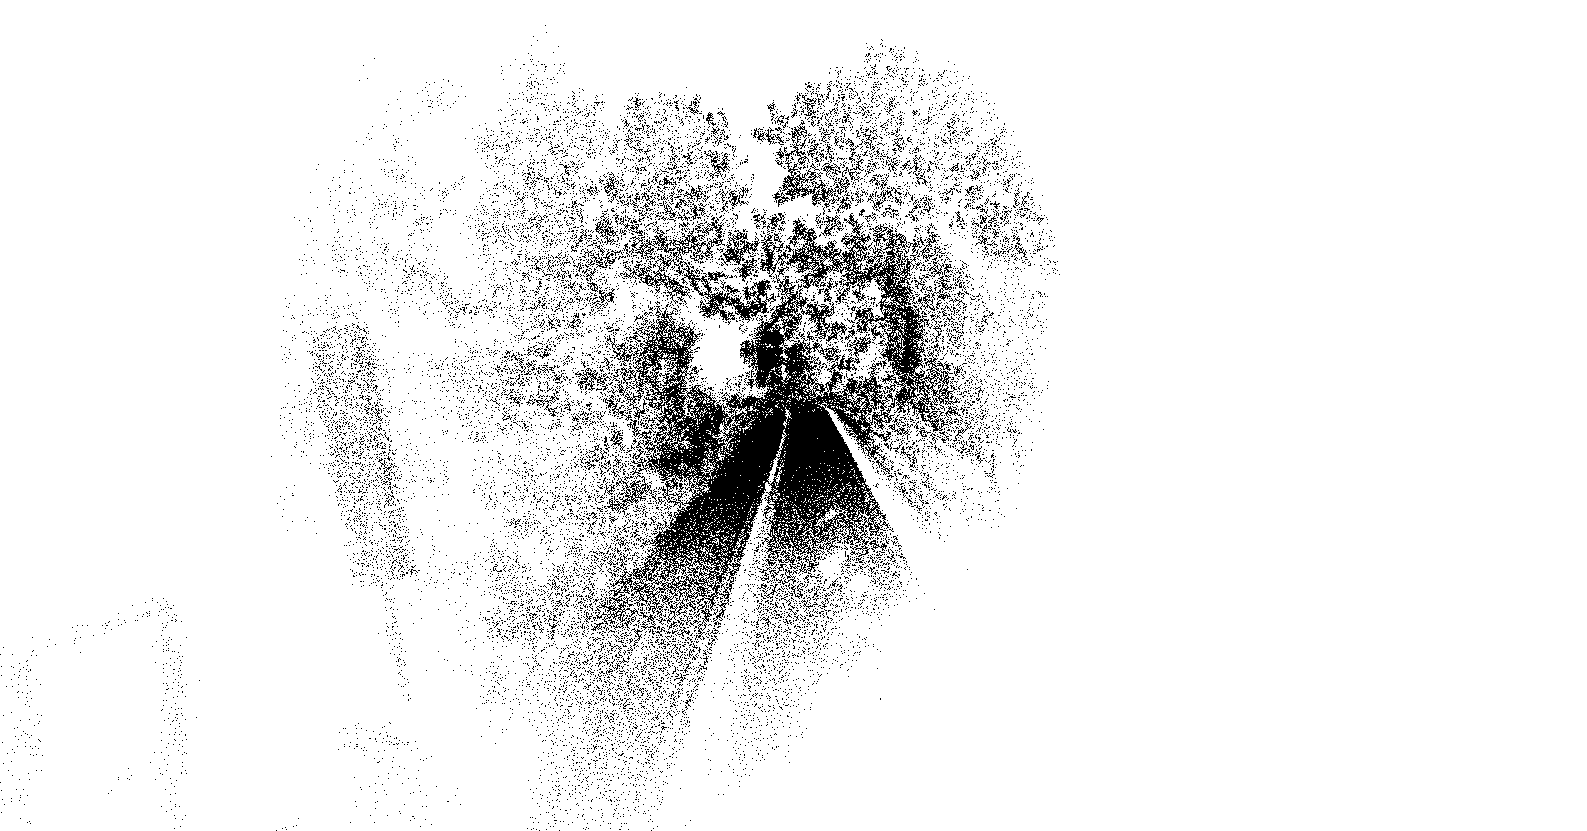
\includegraphics[width=0.95\linewidth]{obrazky-figures/referencny_obrazok.png}
    \caption{Referenčný obrázok, ktorý bol dodaný na začiatku práce spolu s~mračnom bodov a údajmi o~pohybe kamery v~ňom. Obrázok je tu pre lepšiu viditeľnosť s~invertovanými farbami a zväčšeným kontrastom.}
    \label{fig:referencny-obrazok}
\end{figure}

Cieľom tejto prvotnej fázy bolo najmä oboznámenie sa s~dátami a základnými princípmi vykresľovania bodov. Výsledky, ktoré sa nakoniec podarilo dosiahnuť, boli podobné referenčným obrázkom, aj keď nie úplne identické. Ukázalo sa, že údaje o~pohybe kamery majú iný súradnicový systém ako mračno bodov (líšilo sa poradie ôs) a že je potrebné pridať isté posunutie a otočenie, aby sa výsledky podobali referenčným obrázkom (posunutie kamery do stredu vlaku, podľa dodaných dát bola naľavo od stredu).

Ďalej už nasledovala práca s~existujúcimi knižnicami a frameworkami v~jazyku Python. Prvotným plánom bolo použiť knižnicu Pydeck (pre vizualizáciu dát) s~frameworkom Streamlit (pre tvorbu GUI). Pydeck bol zvolený preto, že je nadstavbou nad javascriptovým frameworkom deck.gl, ktorý pri vykresľovaní dát využíva hardwarovú akceleráciu (GPU) a má dobrú výkonnosť. Ukázalo sa však, že Streamlit nepodporuje Pydeck v~plnej miere, a teda sa nedá využiť. Preto bol namiesto Streamlitu použitý framework Dash, ktorý už mal podporu pre Pydeck dostatočnú.

Pomocou tohto frameworku bola vytvorená jednoduchá webová aplikácia zobrazujúca ukážkové dáta a umožňujúca základné nastavenia vzhľadu. Do tejto aplikácie bolo zahrnuté aj zobrazovanie kamerového záznamu, pre tento účel bolo provizórne použité video z~prejazdu tej istej trate natočené v~roku 2012. Pri tom sa zistilo, že vykresľovanie dát pomocou kombinácie knižníc Pydeck a Dash Deck tak, ako je to vo vzorových príkladoch v~dokumentácii knižnice Dash Deck, je značne neefektívne. Jedno vykreslenie mračna bodov zaberalo zhruba 3 sekundy, čo bolo spôsobené transformáciami medzi rôznymi formátmi, ako to bolo popísané v~sekcii \ref{sec:deck_gl}.

Tento čas sa podarilo významne zredukovať použitím knižnice Dash Deck bez knižnice Pydeck. Výsledok však stále nebol dosť dobrý na to, aby mohla hladko bežať animácia pohybu vlaku, a ani napriek rôznym pokusom sa ho už nepodarilo v~rámci tejto kombinácie technológií vo významnejšej miere vylepšiť. Čas vykreslenia mračna bodov bol pritom úmerný počtu bodov a príčina neefektivity bola v~spôsobe implementácie knižnice Dash Deck. Bolo navyše potrebné rátať s~tým, že aplikácia bude zaťažená aj zobrazovaním videa. Preto bolo rozhodnuté optimalizovať vykresľovanie dát vynechaním knižnice Dash Deck a použitím frameworku deck.gl priamo z~jazyka Javascript.

\section{Optimalizácia vykresľovania mračna bodov priamym použitím jazyka JavaScript}

Pythonový framework Dash interne používa na vytváranie používateľského rozhrania JavaScript, konkrétne framework React \cite{dash_documentation}. Jeho tvorcovia rátali s~tým, že vývojári, ktorí ho budú používať, budú niekedy chcieť priamo použiť javascriptový kód. Preto to tento framework umožňuje viacerými spôsobmi:

\begin{itemize}
    \item Klientske callbacky. Podobajú sa tým štandardným, ale na rozdiel od nich bežia iba na klientovi a píšu sa v~jazyku JavaScript. Štandardné callbacky bežia na serveri a píšu sa v~Pythone.
    \item Skripty v~jazyku JavaScript, ktoré je možné pripojiť k~generovanej HTML stránke. Spustia sa automaticky pri otvorení stránky v~prehliadači.
    \item Vytváranie vlastných komponentov používateľského rozhrania pomocou frameworku React.
\end{itemize}

V~tejto práci bola pre jednoduchosť využitá prvá a druhá možnosť. Bol napísaný skript \texttt{visualisation.js}, v~ktorom sú definované funkcie pre zobrazenie a zmeny zobrazenia dát pomocou deck.gl. Odkazy na tieto funkcie sú potom priradené do objektu \texttt{window}, aby bolo možné volať ich z~klientskych callbackov. Tento objekt teda tvorí rozhranie skriptu \texttt{visualisation.js}, ktoré je využívané zvyškom kódu aplikácie.

Pre správne pripojenie zdrojových kódov frameworku deck.gl k~javascriptovému kódu tak, aby mohol fungovať v~rámci aplikácie napísanej vo frameworku Dash, je nutné použiť bundler. V~rámci tejto práce bol použitý bundler Webpack. Výstupnému skriptu je potrebné nastaviť príponu \texttt{.mjs}, aby ho Dash spustil ako modul.

Meranie výkonnosti vykresľovania mračna bodov pred a po optimalizácii je popísané v~tabuľkách \ref{tab:js_optimalizacia_pred} a \ref{tab:js_optimalizacia_po}.

\begin{table}[h]
    \centering
    \begin{tabular}{>{\centering\arraybackslash}m{10em}|>{\centering\arraybackslash}m{13em}|>{\centering\arraybackslash}m{12em}}
        {\RaggedRight Nastavenie parametra \texttt{interval} [ms]} &  {\RaggedRight Čas, za ktorý prebehla celá animácia (100 snímok) [s]} & {\RaggedRight Priemerný čas vykreslenia jedného snímku [ms]} \\ \hline
        1000 & 101 & 1010 \\
        800 & 80 & 800 \\
        750 & 76 & 760 \\
        700 & 72 & 720 \\
        650 & 71 & 710 \\
        600 & 70 & 700 \\
    \end{tabular}
    \caption{Výkonnosť vykresľovania mračna bodov obsahujúceho 201~880 bodov \textbf{pred optimalizáciou}, teda iba pomocou kódu v~jazyku Python. Použité technológie: Python, Dash, Dash Deck. Z~nameraných údajov vyplýva, že minimálny čas potrebný vykreslenie jednej snímky je asi 750~ms, čo znamená, že rýchlosť nedosahuje ani 2 snímky za sekundu.}
    \label{tab:js_optimalizacia_pred}
\end{table}

\begin{table}[h]
    \centering
    \begin{tabular}{>{\centering\arraybackslash}m{10em}|>{\centering\arraybackslash}m{13em}|>{\centering\arraybackslash}m{12em}}
         Nastavenie parametra \texttt{interval} [ms] &  Čas, za ktorý prebehla celá animácia (500 snímok) [s] & Priemerný čas vykreslenia jedného snímku [ms] \\ \hline
        250 & 126 & 252 \\
        200 & 101 & 202 \\
        150 & 76 & 152 \\
        125 & 68 & 136 \\
        100 & 63 & 126 \\
         75 & 62 & 124 \\
    \end{tabular}
    \caption{Výkonnosť vykresľovania mračna bodov obsahujúceho 201~880 bodov \textbf{po optimalizácii}, teda s~vykresľovaním dát v~jazyku Javascript. Použité technológie: Python, Dash, Javascript, deck.gl. Z~nameraných údajov vyplýva, že minimálny čas potrebný vykreslenie jednej snímky je asi 150~ms, čo zodpovedá rýchlosti asi 6 snímok za sekundu.}
    \label{tab:js_optimalizacia_po}
\end{table}

Riadenie animácie pomocou komponentu \texttt{Interval} frameworku Dash je pomerne ťažkopádne, pretože funguje na základe komunikácie medzi klientom a serverom a tým animáciu spomaľuje. Preto by bolo vhodné ho niečím nahradiť, napríklad riadením animácie v~Javascripte iba na klientskej strane.



\section{Experimenty a vyhodnotenie výsledkov}

\chapter{Záver}


%===============================================================================

% Pro kompilaci po částech (viz projekt.tex) nutno odkomentovat
%\end{document}

